\documentclass[10pt,a4paper]{article}
\usepackage[margin=16mm]{geometry}
\usepackage{xcolor,tabularx,array,booktabs,hyperref,lmodern,microtype,graphicx,tikz,fancyhdr}
\definecolor{ink}{HTML}{17394B}\definecolor{teal}{HTML}{138774}\definecolor{pale}{HTML}{EDF5F1}\definecolor{muted}{HTML}{52646D}
\hypersetup{colorlinks=true,urlcolor=teal,pdftitle={Crystal representation benchmark: first result},pdfauthor={ChimiaLabs}}
\setlength{\parindent}{0pt}\setlength{\parskip}{5pt}\renewcommand{\arraystretch}{1.13}
\pagestyle{fancy}\fancyhf{}\renewcommand{\headrulewidth}{0pt}
\fancyfoot[L]{\scriptsize\color{muted}CHIMIALABS / PUBLIC BENCHMARK / 25 OCTOBER 2026}
\fancyfoot[R]{\scriptsize\color{muted}\thepage\ / 2}
\newcommand{\labeltext}[1]{{\sffamily\bfseries\color{teal}#1}}
\newcommand{\callout}[1]{\colorbox{pale}{\parbox{\dimexpr\linewidth-2\fboxsep\relax}{#1}}}
\begin{document}
{\sffamily\small\color{teal} GENERIC PERIODIC OCCUPATION / VERSION 0.1.1}\par
{\LARGE\bfseries\color{ink} One external geometry test.\\An inspectable numerical foundation.}\par
\callout{\textbf{The generic representation preserves the declared diffraction amplitudes.}\newline Six synthetic transformations, four occupation fixtures and one public titanate CIF have been evaluated. Measured structure identification remains unassessed.}

\begin{tabularx}{\linewidth}{@{}>{\raggedright\arraybackslash\bfseries\color{ink}}p{30mm} X@{}}
\toprule
Generic core & Explicit sites, species, occupancies, row-basis cells, integer supercells, source/tile mappings, exact species counts and supplied periodic exclusion witnesses. \textbf{47 implementation tests pass.}\\
\midrule
Independent controls & Rational cosets and scalar complex sums check six transforms. Four ring fixtures test equal means, different correlations, periodic exclusions and ambiguity. \textbf{57 checks pass; two are not applicable.}\\
\midrule
External CIF & A21am layered titanate: \textbf{60 site/species records}, including mixed Ca/Sr alternatives; \textbf{48 occupancy-weighted atoms}. Literal composition and CIF round trips retained.\\
\midrule
Forward agreement & Across \textbf{2,197 reciprocal vectors}, parent amplitudes agree with Gemmi's separate calculator to a maximum absolute error of \textbf{$4.08\times10^{-13}$}. Two nontrivial supercells pass complete declared grids.\\
\bottomrule
\end{tabularx}

\textbf{Scope of that agreement.} The source contains no ADPs. Calculations deliberately use zero ADPs, neutral IT92 X-ray factors and no anomalous terms. Gemmi supplies symmetry admission and the common factor tables; its calculator is independently implemented, but the crystallographic inputs are shared. No fitted scale or background repairs are used.

\labeltext{The occupation controls also preserve ambiguity}\par
\begin{center}
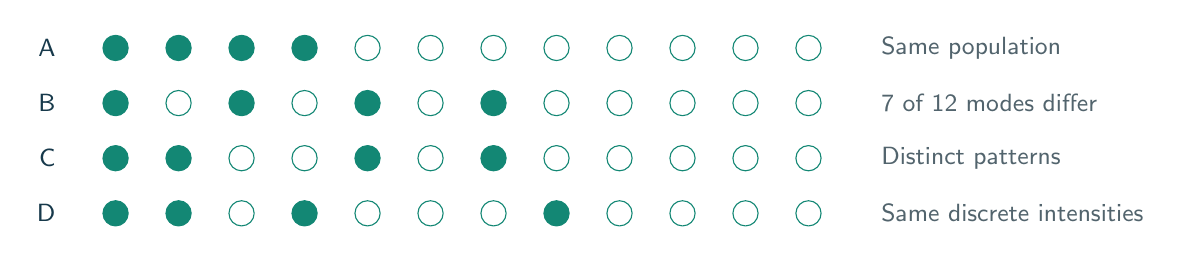
\begin{tikzpicture}[x=8mm,y=7mm,font=\sffamily\small]
\foreach \r/\label in {0/A,1/B,2/C,3/D}{
\node[anchor=east,color=ink] at (-.8,-\r) {\label};
\foreach \i in {0,...,11}{\draw[teal,fill=white] (\i,-\r) circle (1.6mm);}}
\foreach \i in {0,1,2,3}{\fill[teal] (\i,0) circle (1.6mm);}
\foreach \i in {0,2,4,6}{\fill[teal] (\i,-1) circle (1.6mm);}
\foreach \i in {0,1,4,6}{\fill[teal] (\i,-2) circle (1.6mm);}
\foreach \i in {0,1,3,7}{\fill[teal] (\i,-3) circle (1.6mm);}
\node[anchor=west,color=muted] at (12,0) {Same population};
\node[anchor=west,color=muted] at (12,-1) {7 of 12 modes differ};
\node[anchor=west,color=muted] at (12,-2) {Distinct patterns};
\node[anchor=west,color=muted] at (12,-3) {Same discrete intensities};
\end{tikzpicture}
\end{center}
{\small Each row occupies four positions on a periodic twelve-site ring. Exhaustive integer enumeration of all \textbf{495} configurations confirms C/D share cyclic autocorrelation but are not related by translation or reversal. This is a discrete periodic mathematical result, not a chemical or powder-uniqueness claim.}

\labeltext{A correction preserved, and a claim narrowed}\par
Run001 passed its finite controls. Review then exposed large-coordinate numerical errors outside those fixtures. Its exact source/result remain archived. Version 0.1.1 corrects phase evaluation and expansion and passes revalidation. Under the published protocol, \textbf{VT07 is now development data for this revision}; a fresh material is needed for the next held-out test. Neither run was blinded discovery.

\labeltext{What remains before an experimental claim}\par
The deposited TOPAS input is a different P21nm multiphase model and references an absent XYE filename. Full-profile reproduction needs a matched model, observations, ADPs and response. Next: admit a new occupational family, freeze the corrected core, then evaluate. Fe$_7$S$_8$ is a candidate whose structure/instrument inputs remain unresolved.

{\footnotesize\color{muted}\href{https://github.com/xchemtina/chimialabs-osi-2026/tree/generalization-20261025/benchmark}{Code, protocol, amendments and numerical receipts}\quad /\quad \href{https://gemmi.readthedocs.io/en/stable/scattering.html}{Gemmi scattering conventions}. Editable sources and exact environment are included. No private structures or legacy private code are in this package.}

\newpage
{\sffamily\small\color{teal} DATA ADMISSION / RUST POWDER PLOT}\par
{\LARGE\bfseries\color{ink} The measurements available for the next test}\par
{\small Five deposited Diamond I11 observations, 75,000 points each. This is a source-data view, not a fit or a phase assignment. Temperatures are taken from deposit folder labels.}
\begin{center}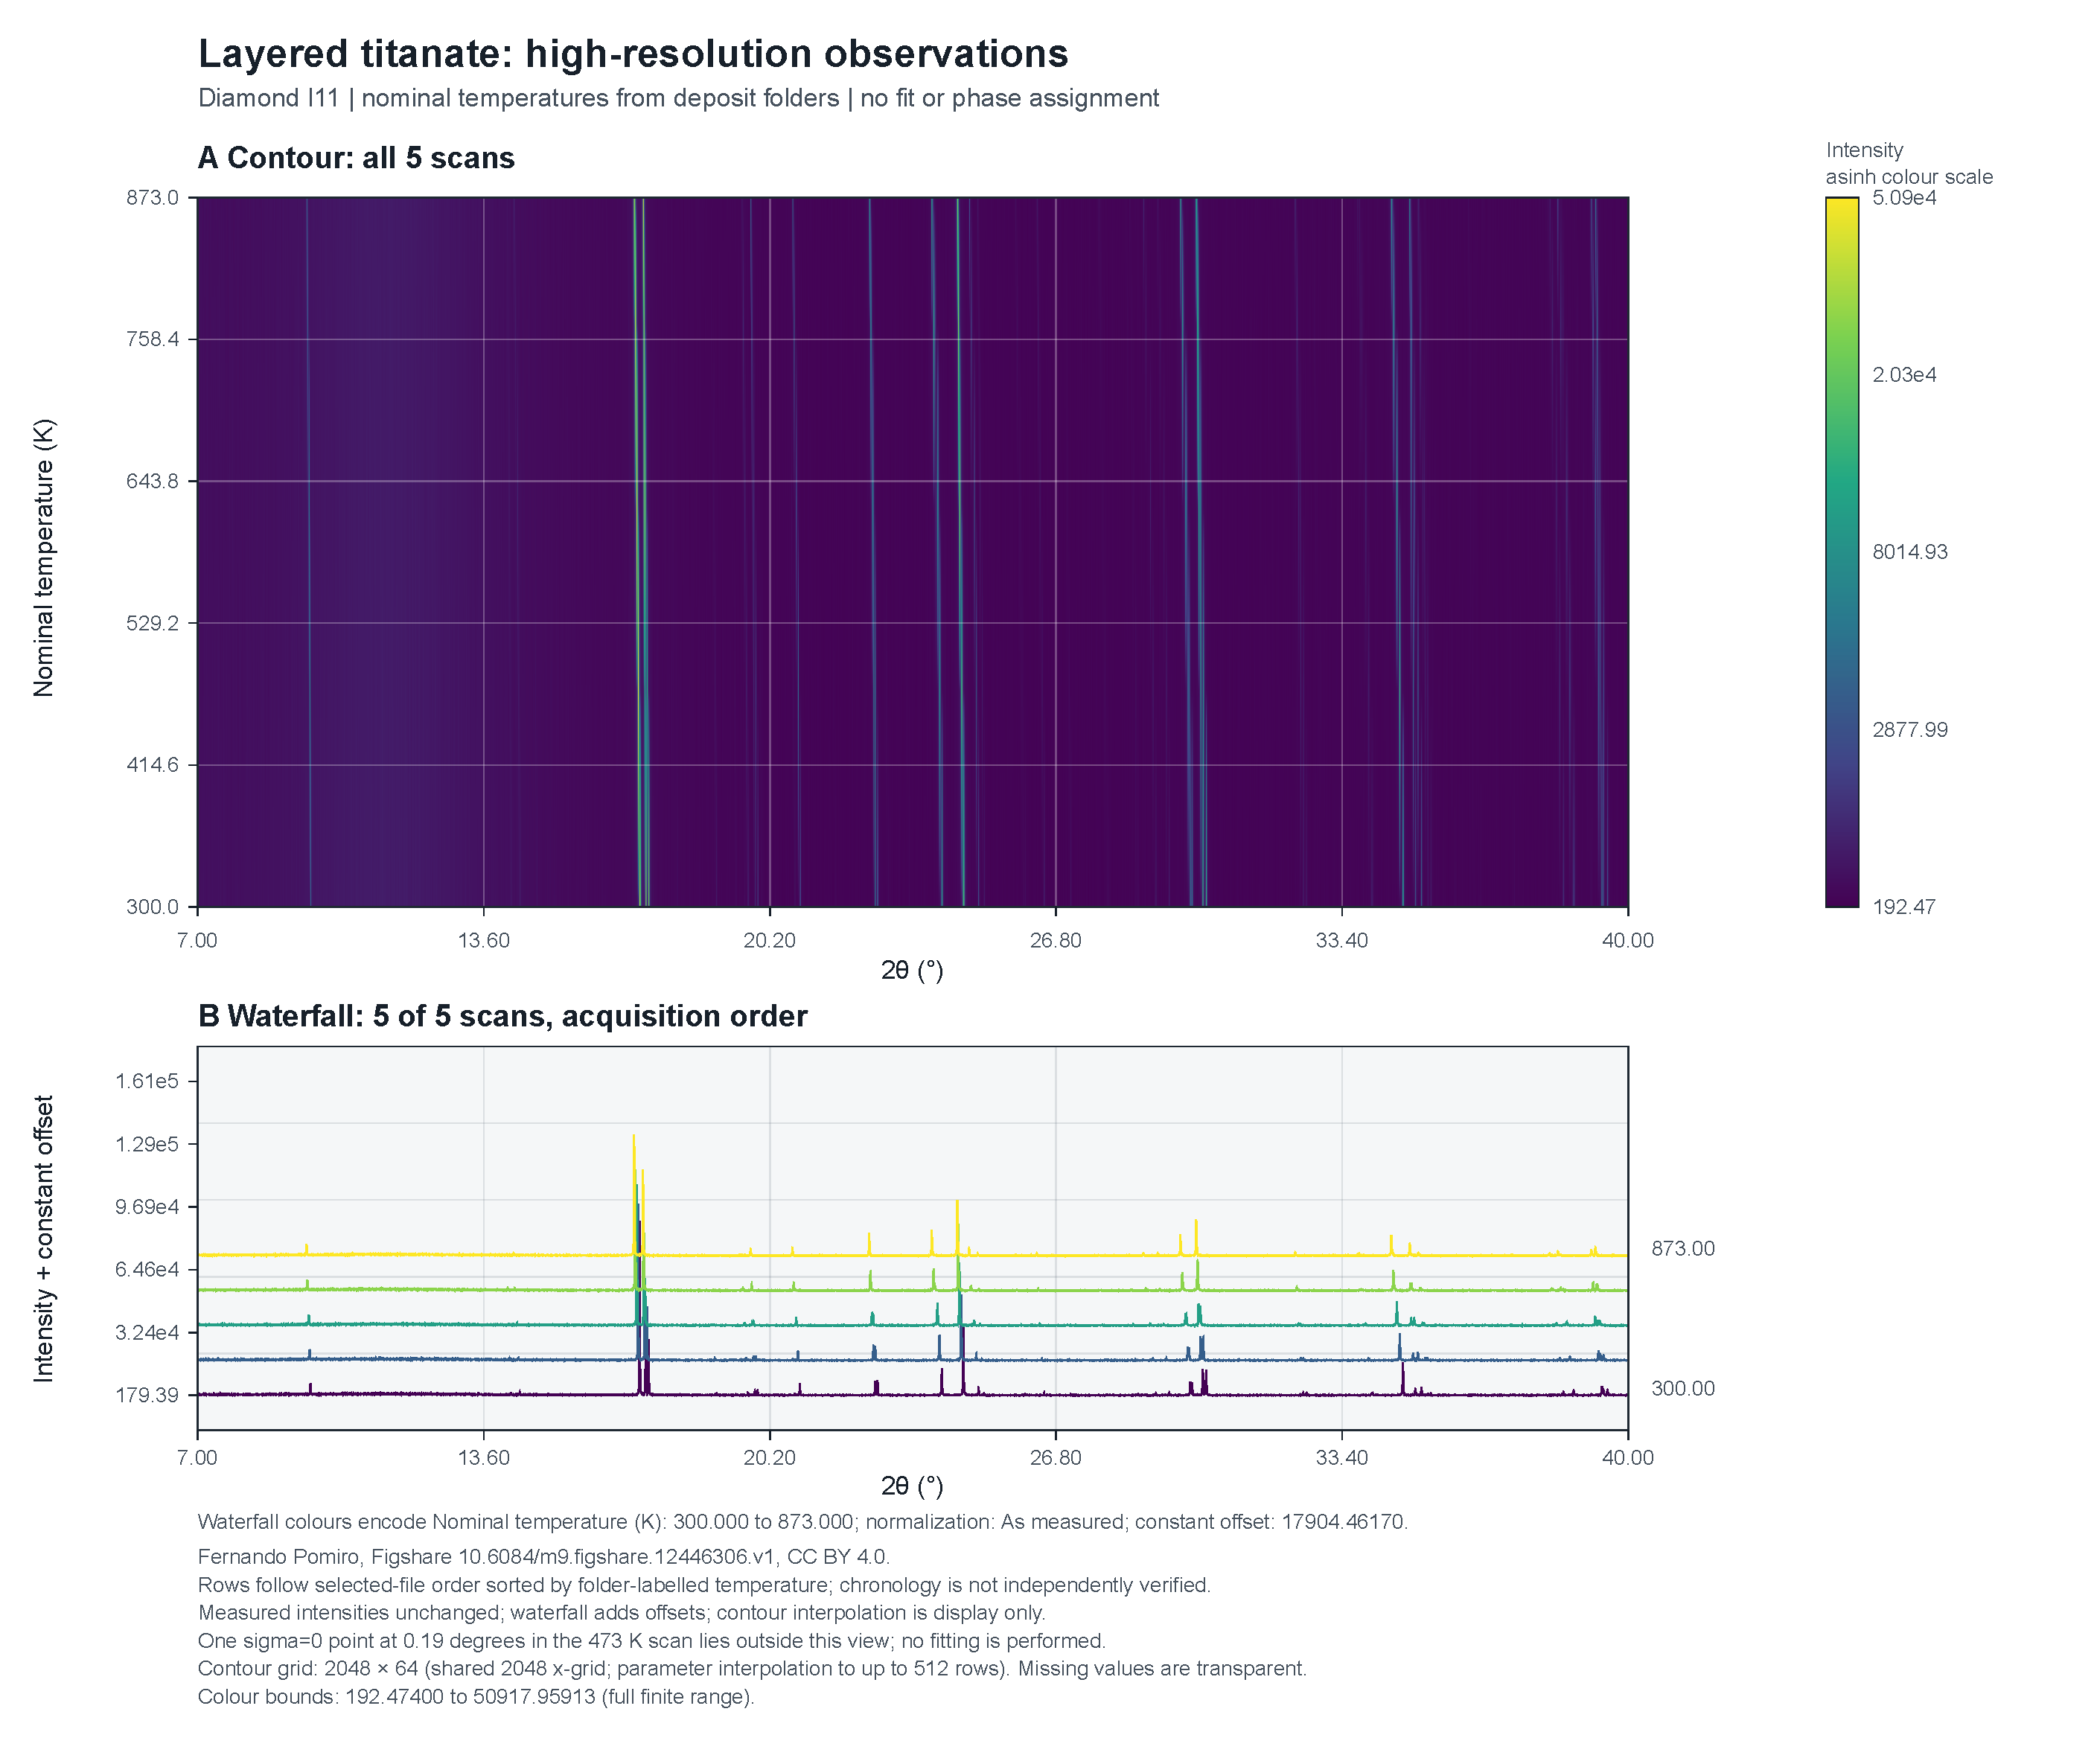
\includegraphics[width=\linewidth]{../figures/vt07-series-v2.pdf}\end{center}
\labeltext{Rendered with Rust Powder Plot}\par
Original intensities are preserved. Waterfall offsets and contour interpolation are display operations. The renderer's fixed ``acquisition order'' heading denotes the selected file order here; chronology has not been independently verified. One zero-sigma point at $0.19^\circ$ in the 473 K scan lies outside this view and is not admitted to a weighted fit.

{\small Source: Fernando Pomiro (2020), \emph{Cif\_files\_and\_exp\_data.zip}, \href{https://doi.org/10.6084/m9.figshare.12446306.v1}{Figshare DOI 10.6084/m9.figshare.12446306.v1}, \href{https://creativecommons.org/licenses/by/4.0/}{CC BY 4.0}. Native SVG, PDF/PNG conversions, input identities and a regeneration command are supplied. The plotted observations are distinct from the fixed-model amplitude controls on page 1.}
\end{document}
